\refstepcounter{figure}
\noindent Figure \thefigure\ shows packets received.

\begin{center}
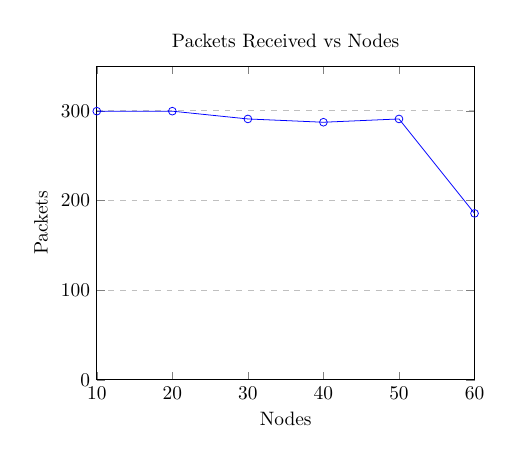
\begin{tikzpicture}[scale=0.7]
\begin{axis}[
title={Packets Received vs Nodes},
xlabel={Nodes}, ylabel={Packets},
xmin=10, xmax=60, ymin=0, ymax=350,
xtick={10,20,30,40,50,60},
ymajorgrids=true, grid style=dashed,
]

\addplot[color=blue, mark=o] coordinates {(10,299.67) (20,299.67) (30,291) (40,287.33) (50,291) (60,185.67)};

\end{axis}
\end{tikzpicture}

\textbf{Figure \thefigure: Packets Received vs Nodes}
\label{fig:packets_density}
\end{center}